\documentclass{article}

% --- OVERLEAF COMPATIBLE PREAMBLE ---
\usepackage[margin=1in]{geometry}
\usepackage[utf8]{inputenc}
\usepackage[T1]{fontenc}
\usepackage[english]{babel}
\usepackage{graphicx}

% Set font to Sans Serif (Helvetica) to approximate Calibri
\usepackage{helvet}
\renewcommand{\familydefault}{\sfdefault}

% --- USER SPECIFIC PACKAGES ---
\usepackage{amsmath}
\usepackage{amssymb}
\usepackage{booktabs}
\usepackage{xcolor}
\usepackage{colortbl}
\usepackage{float}
\usepackage{subcaption}
\usepackage{parskip} % paragraph spacing
\setlength{\parskip}{1em}
\hyphenpenalty=10000
\exhyphenpenalty=10000
\emergencystretch=3em

% Reduce spacing around and between floats (tables)
\setlength{\floatsep}{4pt}
\setlength{\textfloatsep}{8pt}
\setlength{\intextsep}{4pt}

\setcounter{secnumdepth}{0}

% Define custom colors to match the image data
\definecolor{trueyellow}{HTML}{FFFF00}
\definecolor{meangreen}{HTML}{90EE90}
\definecolor{sigmablue}{HTML}{00CED1}
\definecolor{offpurple}{HTML}{DA70D6}

% Legend colors for Misclassification
\definecolor{negchange}{HTML}{808080} % Gray
\definecolor{improved}{HTML}{558B2F} % Dark Green
\definecolor{greatimproved}{HTML}{A5FF7F} % Bright Green
\definecolor{worsened}{HTML}{FF8A8A} % Light Red
\definecolor{greatworsened}{HTML}{8B0000} % Dark Red



% --- DOCUMENT METADATA ---
\title{Programming Assignment 3 \\ \large Eigenfaces for Recognition \\ CS 479}
\author{Jackson Loughmiller}
\date{April 7, 2026}

\begin{document}

% Title and Declaration Page
\begin{titlepage}
    \centering
    \vspace*{\fill}
    
    {\huge \textbf{Programming Assignment 3}} \\
    \vspace{0.5cm}
    {\Large Eigenfaces for Recognition} \\
    \vspace{0.5cm}
    {\large CS 479}
    
    \vspace{2cm}
    
    {\large Jackson Loughmiller} \\
    \vspace{0.2cm}
    {\large May 4, 2026}
    
    \vspace{3cm}
    
    \noindent I declare that all material in this assignment is my own work except
    where there is clear acknowledgment or reference to the work of others.
    I understand that both my report and code may be subjected to plagiarism
    detection software, and fully accept all consequences if found
    responsible for plagiarism, as explained in the syllabus, and described
    in UNR's Academic Standards Policy: UAM 6,502.
    
    \vspace*{\fill}
\end{titlepage}

\newpage

\section{Theory}\label{theory}

\subsection{Experiment a: Face Recognition}\label{experiment-a}

\subsubsection*{Dimensionality Reduction}\label{dimensionality-reduction}

Dimensionality reduction is a technique that is often required in practice due 
to data often having a large number of dimensions, making it computationally expensive to 
compute results and requiring large amounts of data for training. Data with very high 
dimensions incurs the “Curse of Dimensionality”, which states that as the amount of 
dimensions increases, the amount of training data needed increases exponentially. 
Dimensionality reduction seeks to remedy this problem by using either feature extraction 
or feature selection, for this report feature extraction is the only relevant method. 

\subsubsection*{Feature Extraction}\label{feature-extraction}

Feature extraction is a method of dimensionality reduction that creates 
a new, smaller set of features from the original features by performing 
certain transformations. This new set of features is related to the original, 
however they do not correspond to physical features that humans are able to comprehend. 

\subsubsection*{Principle Component Analysis}\label{principle-component-analysis}

Principal component analysis (PCA) is a feature extraction technique used for dimensionality reduction. 
A data point:
\begin{equation}\label{eq:xRD}
    \mathbf{x} \in \mathbb{R}^D
\end{equation}
can be represented as a linear combination of an orthonormal set of D basis vectors:
\begin{equation}\label{eq:lin_combo_D}
    \mathbf{x} = \sum_{i=1}^{D} x_i v_i = x_1 v_1 + x_2 v_2 + \ldots + x_D v_D
\end{equation}
PCA reduces the dimensionality by approximating each vector, x, in a subspace using K<<D orthonormal
basis vectors:

\begin{equation}\label{eq:lin_combo_K}
    \mathbf{x} = \sum_{i=1}^{K} x_i v_i = x_1 v_1 + x_2 v_2 + \ldots + x_K v_K
\end{equation}

It does this by minimizing the function below in Eq. \ref{eq:recon_error}, conceptually the information loss.

\begin{equation}\label{eq:recon_error}
    \| \mathbf{x} - \hat{\mathbf{x}} \|
\end{equation}

Overall, PCA consists of essentially 3 steps: 

\begin{enumerate}
    \item Find the eigenvectors of the covariance matrix of the data.
    \item Sort the eigenvectors with respect to their eigenvalue, essentially sorting by greatest to smallest variance.
    \item Choose the top K eigenvectors, where K is a parameter.
\end{enumerate}

To compute the covariance matrix, one needs to first compute the sample mean, and subtract it from all the data
to center it. This can be done using Eqs. \ref{eq:sample_mean} and \ref{eq:center}, below:

\begin{equation}\label{eq:sample_mean}
    \bar{\mathbf{x}} = \frac{1}{M} \sum_{i=1}^{M} \mathbf{x}_i
\end{equation}
\begin{equation}\label{eq:center}
    \Phi_i = \mathbf{x}_i - \bar{\mathbf{x}}
\end{equation}

The covariance matrix can then be calculated using Eq. \ref{eq:cov_matrix}, below:

\begin{equation}\label{eq:cov_matrix}
    \Sigma_{\mathbf{x}} = \frac{1}{M} \sum_{i=1}^{M} (\mathbf{x}_i - \bar{\mathbf{x}})(\mathbf{x}_i - \bar{\mathbf{x}})^T = \frac{1}{M} \sum_{i=1}^{M} \Phi_i \Phi_i^T = \frac{1}{M} A A^T
\end{equation}

Then, the eigenvectors can be calculated with Eq. \ref{eq:eigen_vectors}, below:

\begin{equation}\label{eq:eigen_vectors}
    \Sigma_x u_i = \lambda_i u_i
\end{equation}

Once the eigenvectors and eigenvalues have been computed, the last step is simply to choose the eigen vectors
associated with the top K eigenvalues. 

For computational efficiency, Eq. \ref{eq:cov_matrix} can be calculated approximately using Eq. \ref{eq:cov_matrix_2}, below: 

\begin{equation}\label{eq:cov_matrix_2}
    A A^T
\end{equation}

It can be shown that Eq. \ref{eq:cov_matrix_2} gives the top M eigenvectors that would be computed from Eq. \ref{eq:cov_matrix}, 
and since PCA needs only the top K eigenvectors, this is perfect for this situation. 

\section{Results and Discussion}\label{results-and-discussion}

\subsection{Experiment a}\label{experiment-a-a}

For experiment a, I used the PCA approach to perform facial recognition, using the 
Mahalanobis distance on the eigenface space projections of query images for classification. Figure \ref{fig:avg_face_a}, below, 
shows a visual representation of the average face that is subtracted from the images to center the data. 
The average face does not capture any truly distinct features, which is expected. 

\begin{figure}[H]
    \centering
    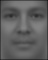
\includegraphics[width=0.25\textwidth]{../experiment_a_results/average_face.jpg}
    \caption{Average face computed from the fa\_H training set.}
    \label{fig:avg_face_a}
\end{figure}

\newpage
Figure \ref{fig:top10_ef}, below, shows the eigenfaces corresponding to the top 10 largest eigenvalues, and figure \ref{fig:bot10_ef}
shows the eigenfaces corresponding to the smallest 10 eigenvalues. 

\begin{figure}[H]
    \centering
    \begin{subfigure}[b]{0.09\textwidth}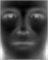
\includegraphics[width=\textwidth]{../eigen_faces_imgs/ef_0.jpg}\end{subfigure}\hfill
    \begin{subfigure}[b]{0.09\textwidth}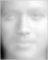
\includegraphics[width=\textwidth]{../eigen_faces_imgs/ef_1.jpg}\end{subfigure}\hfill
    \begin{subfigure}[b]{0.09\textwidth}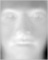
\includegraphics[width=\textwidth]{../eigen_faces_imgs/ef_2.jpg}\end{subfigure}\hfill
    \begin{subfigure}[b]{0.09\textwidth}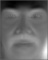
\includegraphics[width=\textwidth]{../eigen_faces_imgs/ef_3.jpg}\end{subfigure}\hfill
    \begin{subfigure}[b]{0.09\textwidth}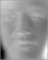
\includegraphics[width=\textwidth]{../eigen_faces_imgs/ef_4.jpg}\end{subfigure}\hfill
    \begin{subfigure}[b]{0.09\textwidth}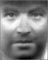
\includegraphics[width=\textwidth]{../eigen_faces_imgs/ef_5.jpg}\end{subfigure}\hfill
    \begin{subfigure}[b]{0.09\textwidth}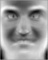
\includegraphics[width=\textwidth]{../eigen_faces_imgs/ef_6.jpg}\end{subfigure}\hfill
    \begin{subfigure}[b]{0.09\textwidth}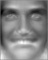
\includegraphics[width=\textwidth]{../eigen_faces_imgs/ef_7.jpg}\end{subfigure}\hfill
    \begin{subfigure}[b]{0.09\textwidth}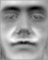
\includegraphics[width=\textwidth]{../eigen_faces_imgs/ef_8.jpg}\end{subfigure}\hfill
    \begin{subfigure}[b]{0.09\textwidth}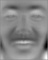
\includegraphics[width=\textwidth]{../eigen_faces_imgs/ef_9.jpg}\end{subfigure}
    \caption{Top 10 eigenfaces corresponding to the 10 largest eigenvalues.}
    \label{fig:top10_ef}
\end{figure}

\begin{figure}[H]
    \centering
    \begin{subfigure}[b]{0.09\textwidth}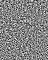
\includegraphics[width=\textwidth]{../eigen_faces_imgs/ef_1194.jpg}\end{subfigure}\hfill
    \begin{subfigure}[b]{0.09\textwidth}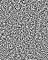
\includegraphics[width=\textwidth]{../eigen_faces_imgs/ef_1195.jpg}\end{subfigure}\hfill
    \begin{subfigure}[b]{0.09\textwidth}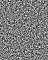
\includegraphics[width=\textwidth]{../eigen_faces_imgs/ef_1196.jpg}\end{subfigure}\hfill
    \begin{subfigure}[b]{0.09\textwidth}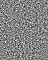
\includegraphics[width=\textwidth]{../eigen_faces_imgs/ef_1197.jpg}\end{subfigure}\hfill
    \begin{subfigure}[b]{0.09\textwidth}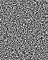
\includegraphics[width=\textwidth]{../eigen_faces_imgs/ef_1198.jpg}\end{subfigure}\hfill
    \begin{subfigure}[b]{0.09\textwidth}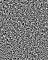
\includegraphics[width=\textwidth]{../eigen_faces_imgs/ef_1199.jpg}\end{subfigure}\hfill
    \begin{subfigure}[b]{0.09\textwidth}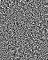
\includegraphics[width=\textwidth]{../eigen_faces_imgs/ef_1200.jpg}\end{subfigure}\hfill
    \begin{subfigure}[b]{0.09\textwidth}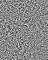
\includegraphics[width=\textwidth]{../eigen_faces_imgs/ef_1201.jpg}\end{subfigure}\hfill
    \begin{subfigure}[b]{0.09\textwidth}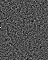
\includegraphics[width=\textwidth]{../eigen_faces_imgs/ef_1202.jpg}\end{subfigure}\hfill
    \begin{subfigure}[b]{0.09\textwidth}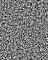
\includegraphics[width=\textwidth]{../eigen_faces_imgs/ef_1203.jpg}\end{subfigure}
    \caption{Bottom 10 eigenfaces corresponding to the 10 smallest eigenvalues.}
    \label{fig:bot10_ef}
\end{figure}

As the figures above show, the top 10 eigenvectors clearly contain more information of the features for a face, showing visible 
facial-like features in their image representations. Due to lack of containing much feature information, and likely also due to 
rounding errors in eigenvalues and eigenvectors calculations, the last 10 images contain what appears to be pure noise from the 
image representations. This makes sense, since the theory behind PCA states the top eigenvectors should contain more information
than the lower ones. 

Figure \ref{fig:cmc}, below, shows the Cumulative Match Characteristic Curve for retaining 80\%, 90\%, and 95\% of the the data during 
classification, plotting rank (number of images within which a classification is considered correct), against the accuracy.
Interestingly, the model seemed to perform approximately the same at high values of rank for 80\% and 90\% of the data, 
however it performed noticeably worse with 95\%. This is likely due to the smaller eigenvalue associated eigenvectors containing less information, 
and potentially being very corrupted with noise from rounding errors. It is notable that with lower rank values (below around 15), 
both 90\% and 95\% work better than 80\%. 

\begin{figure}[H]
    \centering
    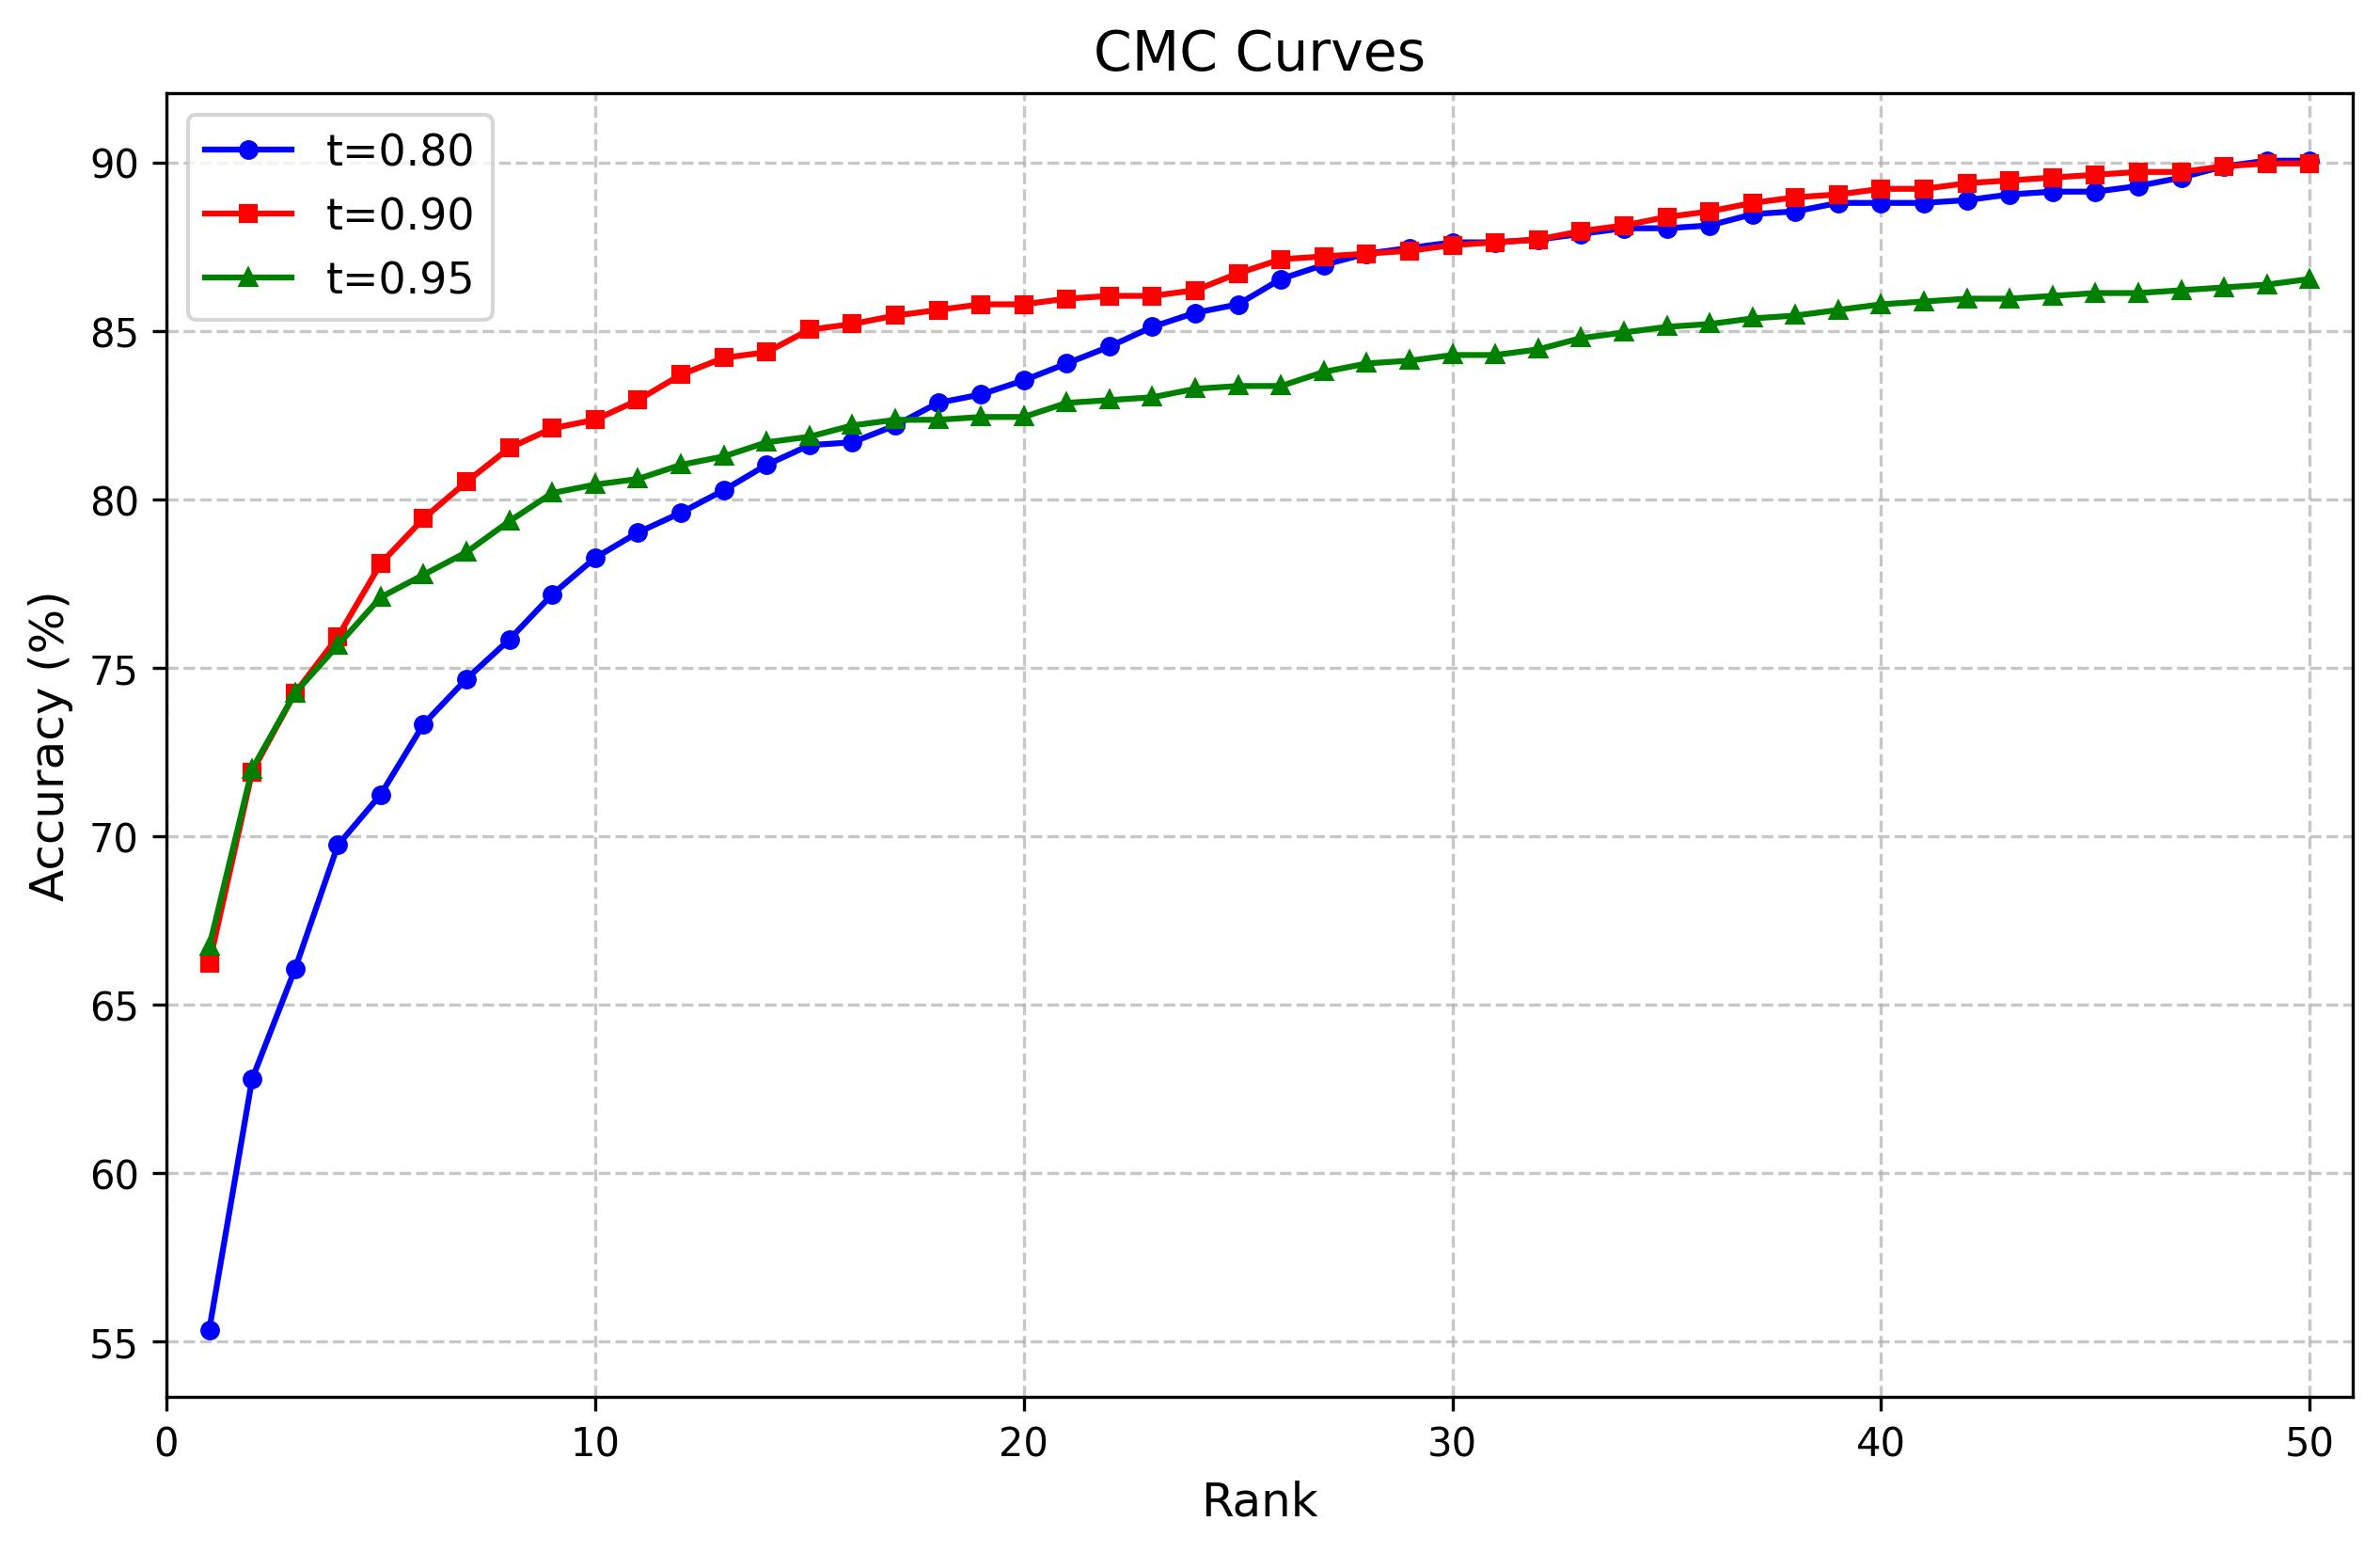
\includegraphics[width=0.8\textwidth]{../Experiment_II.jpg}
    \caption{CMC curves comparing 80\%, 90\%, and 95\% variance thresholds (fa\_H training, fb\_H testing).}
    \label{fig:cmc}
\end{figure}

Figures \ref{fig:correct80} - \ref{fig:incorrect95} show correctly matched and incorrectly matched pairs for different
amounts of information being kept, at 80\%, 90\%, and 95\%. 

\begin{figure}[H]
    \centering
    \begin{subfigure}[b]{0.14\textwidth}\includegraphics[width=\textwidth]{../experiment_a_results/results_80/correct_query_0.jpg}\caption*{Query}\end{subfigure}\hspace{0.3em}
    \begin{subfigure}[b]{0.14\textwidth}\includegraphics[width=\textwidth]{../experiment_a_results/results_80/correct_training_0.jpg}\caption*{Match}\end{subfigure}\hspace{1.5em}
    \begin{subfigure}[b]{0.14\textwidth}\includegraphics[width=\textwidth]{../experiment_a_results/results_80/correct_query_1.jpg}\caption*{Query}\end{subfigure}\hspace{0.3em}
    \begin{subfigure}[b]{0.14\textwidth}\includegraphics[width=\textwidth]{../experiment_a_results/results_80/correct_training_1.jpg}\caption*{Match}\end{subfigure}\hspace{1.5em}
    \begin{subfigure}[b]{0.14\textwidth}\includegraphics[width=\textwidth]{../experiment_a_results/results_80/correct_query_2.jpg}\caption*{Query}\end{subfigure}\hspace{0.3em}
    \begin{subfigure}[b]{0.14\textwidth}\includegraphics[width=\textwidth]{../experiment_a_results/results_80/correct_training_2.jpg}\caption*{Match}\end{subfigure}
    \caption{Three correctly matched query-gallery pairs at 80\% variance threshold (r=1).}
    \label{fig:correct80}
\end{figure}

\begin{figure}[H]
    \centering
    \begin{subfigure}[b]{0.14\textwidth}\includegraphics[width=\textwidth]{../experiment_a_results/results_80/incorrect_query_0.jpg}\caption*{Query}\end{subfigure}\hspace{0.3em}
    \begin{subfigure}[b]{0.14\textwidth}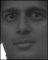
\includegraphics[width=\textwidth]{../experiment_a_results/results_80/incorrect_training_0.jpg}\caption*{Mismatch}\end{subfigure}\hspace{1.5em}
    \begin{subfigure}[b]{0.14\textwidth}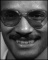
\includegraphics[width=\textwidth]{../experiment_a_results/results_80/incorrect_query_1.jpg}\caption*{Query}\end{subfigure}\hspace{0.3em}
    \begin{subfigure}[b]{0.14\textwidth}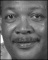
\includegraphics[width=\textwidth]{../experiment_a_results/results_80/incorrect_training_1.jpg}\caption*{Mismatch}\end{subfigure}\hspace{1.5em}
    \begin{subfigure}[b]{0.14\textwidth}\includegraphics[width=\textwidth]{../experiment_a_results/results_80/incorrect_query_2.jpg}\caption*{Query}\end{subfigure}\hspace{0.3em}
    \begin{subfigure}[b]{0.14\textwidth}\includegraphics[width=\textwidth]{../experiment_a_results/results_80/incorrect_training_2.jpg}\caption*{Mismatch}\end{subfigure}
    \caption{Three incorrectly matched query-gallery pairs at 80\% variance threshold (r=1).}
    \label{fig:incorrect80}
\end{figure}

As seen by Figures \ref{fig:correct80} and \ref{fig:incorrect80}, above, even with the mismatched images, the matches seem to have pretty similar
facial features to the query image. Even the pair in which the query image is wearing glasses, the other facial features such as nose shape, 
mustache, and jawline are fairly aligned.  

For both 90\% and 95\% of the data, the mismatches vary more widely from the features seen in the query images. Some of them appear to be somewhat
close at first glance, but upon closer inspection individual features seem much different between query and match. 

\begin{figure}[H]
    \centering
    \begin{subfigure}[b]{0.14\textwidth}\includegraphics[width=\textwidth]{../experiment_a_results/results_90/correct_query_0.jpg}\caption*{Query}\end{subfigure}\hspace{0.3em}
    \begin{subfigure}[b]{0.14\textwidth}\includegraphics[width=\textwidth]{../experiment_a_results/results_90/correct_training_0.jpg}\caption*{Match}\end{subfigure}\hspace{1.5em}
    \begin{subfigure}[b]{0.14\textwidth}\includegraphics[width=\textwidth]{../experiment_a_results/results_90/correct_query_1.jpg}\caption*{Query}\end{subfigure}\hspace{0.3em}
    \begin{subfigure}[b]{0.14\textwidth}\includegraphics[width=\textwidth]{../experiment_a_results/results_90/correct_training_1.jpg}\caption*{Match}\end{subfigure}\hspace{1.5em}
    \begin{subfigure}[b]{0.14\textwidth}\includegraphics[width=\textwidth]{../experiment_a_results/results_90/correct_query_2.jpg}\caption*{Query}\end{subfigure}\hspace{0.3em}
    \begin{subfigure}[b]{0.14\textwidth}\includegraphics[width=\textwidth]{../experiment_a_results/results_90/correct_training_2.jpg}\caption*{Match}\end{subfigure}
    \caption{Three correctly matched query-gallery pairs at 90\% variance threshold (r=1).}
    \label{fig:correct90}
\end{figure}

\begin{figure}[H]
    \centering
    \begin{subfigure}[b]{0.14\textwidth}\includegraphics[width=\textwidth]{../experiment_a_results/results_90/incorrect_query_0.jpg}\caption*{Query}\end{subfigure}\hspace{0.3em}
    \begin{subfigure}[b]{0.14\textwidth}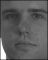
\includegraphics[width=\textwidth]{../experiment_a_results/results_90/incorrect_training_0.jpg}\caption*{Mismatch}\end{subfigure}\hspace{1.5em}
    \begin{subfigure}[b]{0.14\textwidth}\includegraphics[width=\textwidth]{../experiment_a_results/results_90/incorrect_query_1.jpg}\caption*{Query}\end{subfigure}\hspace{0.3em}
    \begin{subfigure}[b]{0.14\textwidth}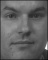
\includegraphics[width=\textwidth]{../experiment_a_results/results_90/incorrect_training_1.jpg}\caption*{Mismatch}\end{subfigure}\hspace{1.5em}
    \begin{subfigure}[b]{0.14\textwidth}\includegraphics[width=\textwidth]{../experiment_a_results/results_90/incorrect_query_2.jpg}\caption*{Query}\end{subfigure}\hspace{0.3em}
    \begin{subfigure}[b]{0.14\textwidth}\includegraphics[width=\textwidth]{../experiment_a_results/results_90/incorrect_training_2.jpg}\caption*{Mismatch}\end{subfigure}
    \caption{Three incorrectly matched query-gallery pairs at 90\% variance threshold (r=1).}
    \label{fig:incorrect90}
\end{figure}

For 95\% of the data in particular, the features have a lot of variance between query and match in the incorrect matches, Figure \ref{fig:incorrect95}. 
In most of the images, at least one prominent feature such as nose shape, eyebrow size, or eye structure are significantly different from the query image. 

\begin{figure}[H]
    \centering
    \begin{subfigure}[b]{0.14\textwidth}\includegraphics[width=\textwidth]{../experiment_a_results/results_95/correct_query_0.jpg}\caption*{Query}\end{subfigure}\hspace{0.3em}
    \begin{subfigure}[b]{0.14\textwidth}\includegraphics[width=\textwidth]{../experiment_a_results/results_95/correct_training_0.jpg}\caption*{Match}\end{subfigure}\hspace{1.5em}
    \begin{subfigure}[b]{0.14\textwidth}\includegraphics[width=\textwidth]{../experiment_a_results/results_95/correct_query_1.jpg}\caption*{Query}\end{subfigure}\hspace{0.3em}
    \begin{subfigure}[b]{0.14\textwidth}\includegraphics[width=\textwidth]{../experiment_a_results/results_95/correct_training_1.jpg}\caption*{Match}\end{subfigure}\hspace{1.5em}
    \begin{subfigure}[b]{0.14\textwidth}\includegraphics[width=\textwidth]{../experiment_a_results/results_95/correct_query_2.jpg}\caption*{Query}\end{subfigure}\hspace{0.3em}
    \begin{subfigure}[b]{0.14\textwidth}\includegraphics[width=\textwidth]{../experiment_a_results/results_95/correct_training_2.jpg}\caption*{Match}\end{subfigure}
    \caption{Three correctly matched query-gallery pairs at 95\% variance threshold (r=1).}
    \label{fig:correct95}
\end{figure}

\begin{figure}[H]
    \centering
    \begin{subfigure}[b]{0.14\textwidth}\includegraphics[width=\textwidth]{../experiment_a_results/results_95/incorrect_query_0.jpg}\caption*{Query}\end{subfigure}\hspace{0.3em}
    \begin{subfigure}[b]{0.14\textwidth}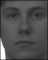
\includegraphics[width=\textwidth]{../experiment_a_results/results_95/incorrect_training_0.jpg}\caption*{Mismatch}\end{subfigure}\hspace{1.5em}
    \begin{subfigure}[b]{0.14\textwidth}\includegraphics[width=\textwidth]{../experiment_a_results/results_95/incorrect_query_1.jpg}\caption*{Query}\end{subfigure}\hspace{0.3em}
    \begin{subfigure}[b]{0.14\textwidth}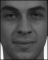
\includegraphics[width=\textwidth]{../experiment_a_results/results_95/incorrect_training_1.jpg}\caption*{Mismatch}\end{subfigure}\hspace{1.5em}
    \begin{subfigure}[b]{0.14\textwidth}\includegraphics[width=\textwidth]{../experiment_a_results/results_95/incorrect_query_2.jpg}\caption*{Query}\end{subfigure}\hspace{0.3em}
    \begin{subfigure}[b]{0.14\textwidth}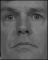
\includegraphics[width=\textwidth]{../experiment_a_results/results_95/incorrect_training_2.jpg}\caption*{Mismatch}\end{subfigure}
    \caption{Three incorrectly matched query-gallery pairs at 95\% variance threshold (r=1).}
    \label{fig:incorrect95}
\end{figure}

These results from the incorrect matches are somewhat unexpected. I expected the 80\% information experiment to produces significantly worse, or more noticeably different
incorrect matches, than the others based on the data seen in the CMC curve. I suspect that the lower accuracy shown in the CMC curve may be due to features being 
included that are not very visible to the human eye in the 90\% and 95\% categories, and are therefore not noticeable in the images. 

\newpage
\subsection{Experiment b}\label{experiment-b-b}

In experiment b, I tested the models performance dealing with intruders, query images of a face that is not in the 
database. To do this, I implemented a threshold value, for which if the distance the model output for the Mahalanobis distance
was larger than the threshold, the query image would be rejected. Figure \ref{fig:roc}, below, shows the ROC curve for different
values of the threshold. I varied the threshold from 0 - 1.24, the maximum distance the model would output based on the data
in the testing set. As seen by the curve, the model outputs more false postives as the threshold increases, which makes
sense given the model would be allowing larger distances to reflect a match. True positives increases up until a point, 
after which the true positives stay relatively the same, while false positives continue to increase. This point likely reflects 
the tipping point at which the model stops having correct matches with larger distances, and instead is just outputting incorrect
matches. 

\begin{figure}[H]
    \centering
    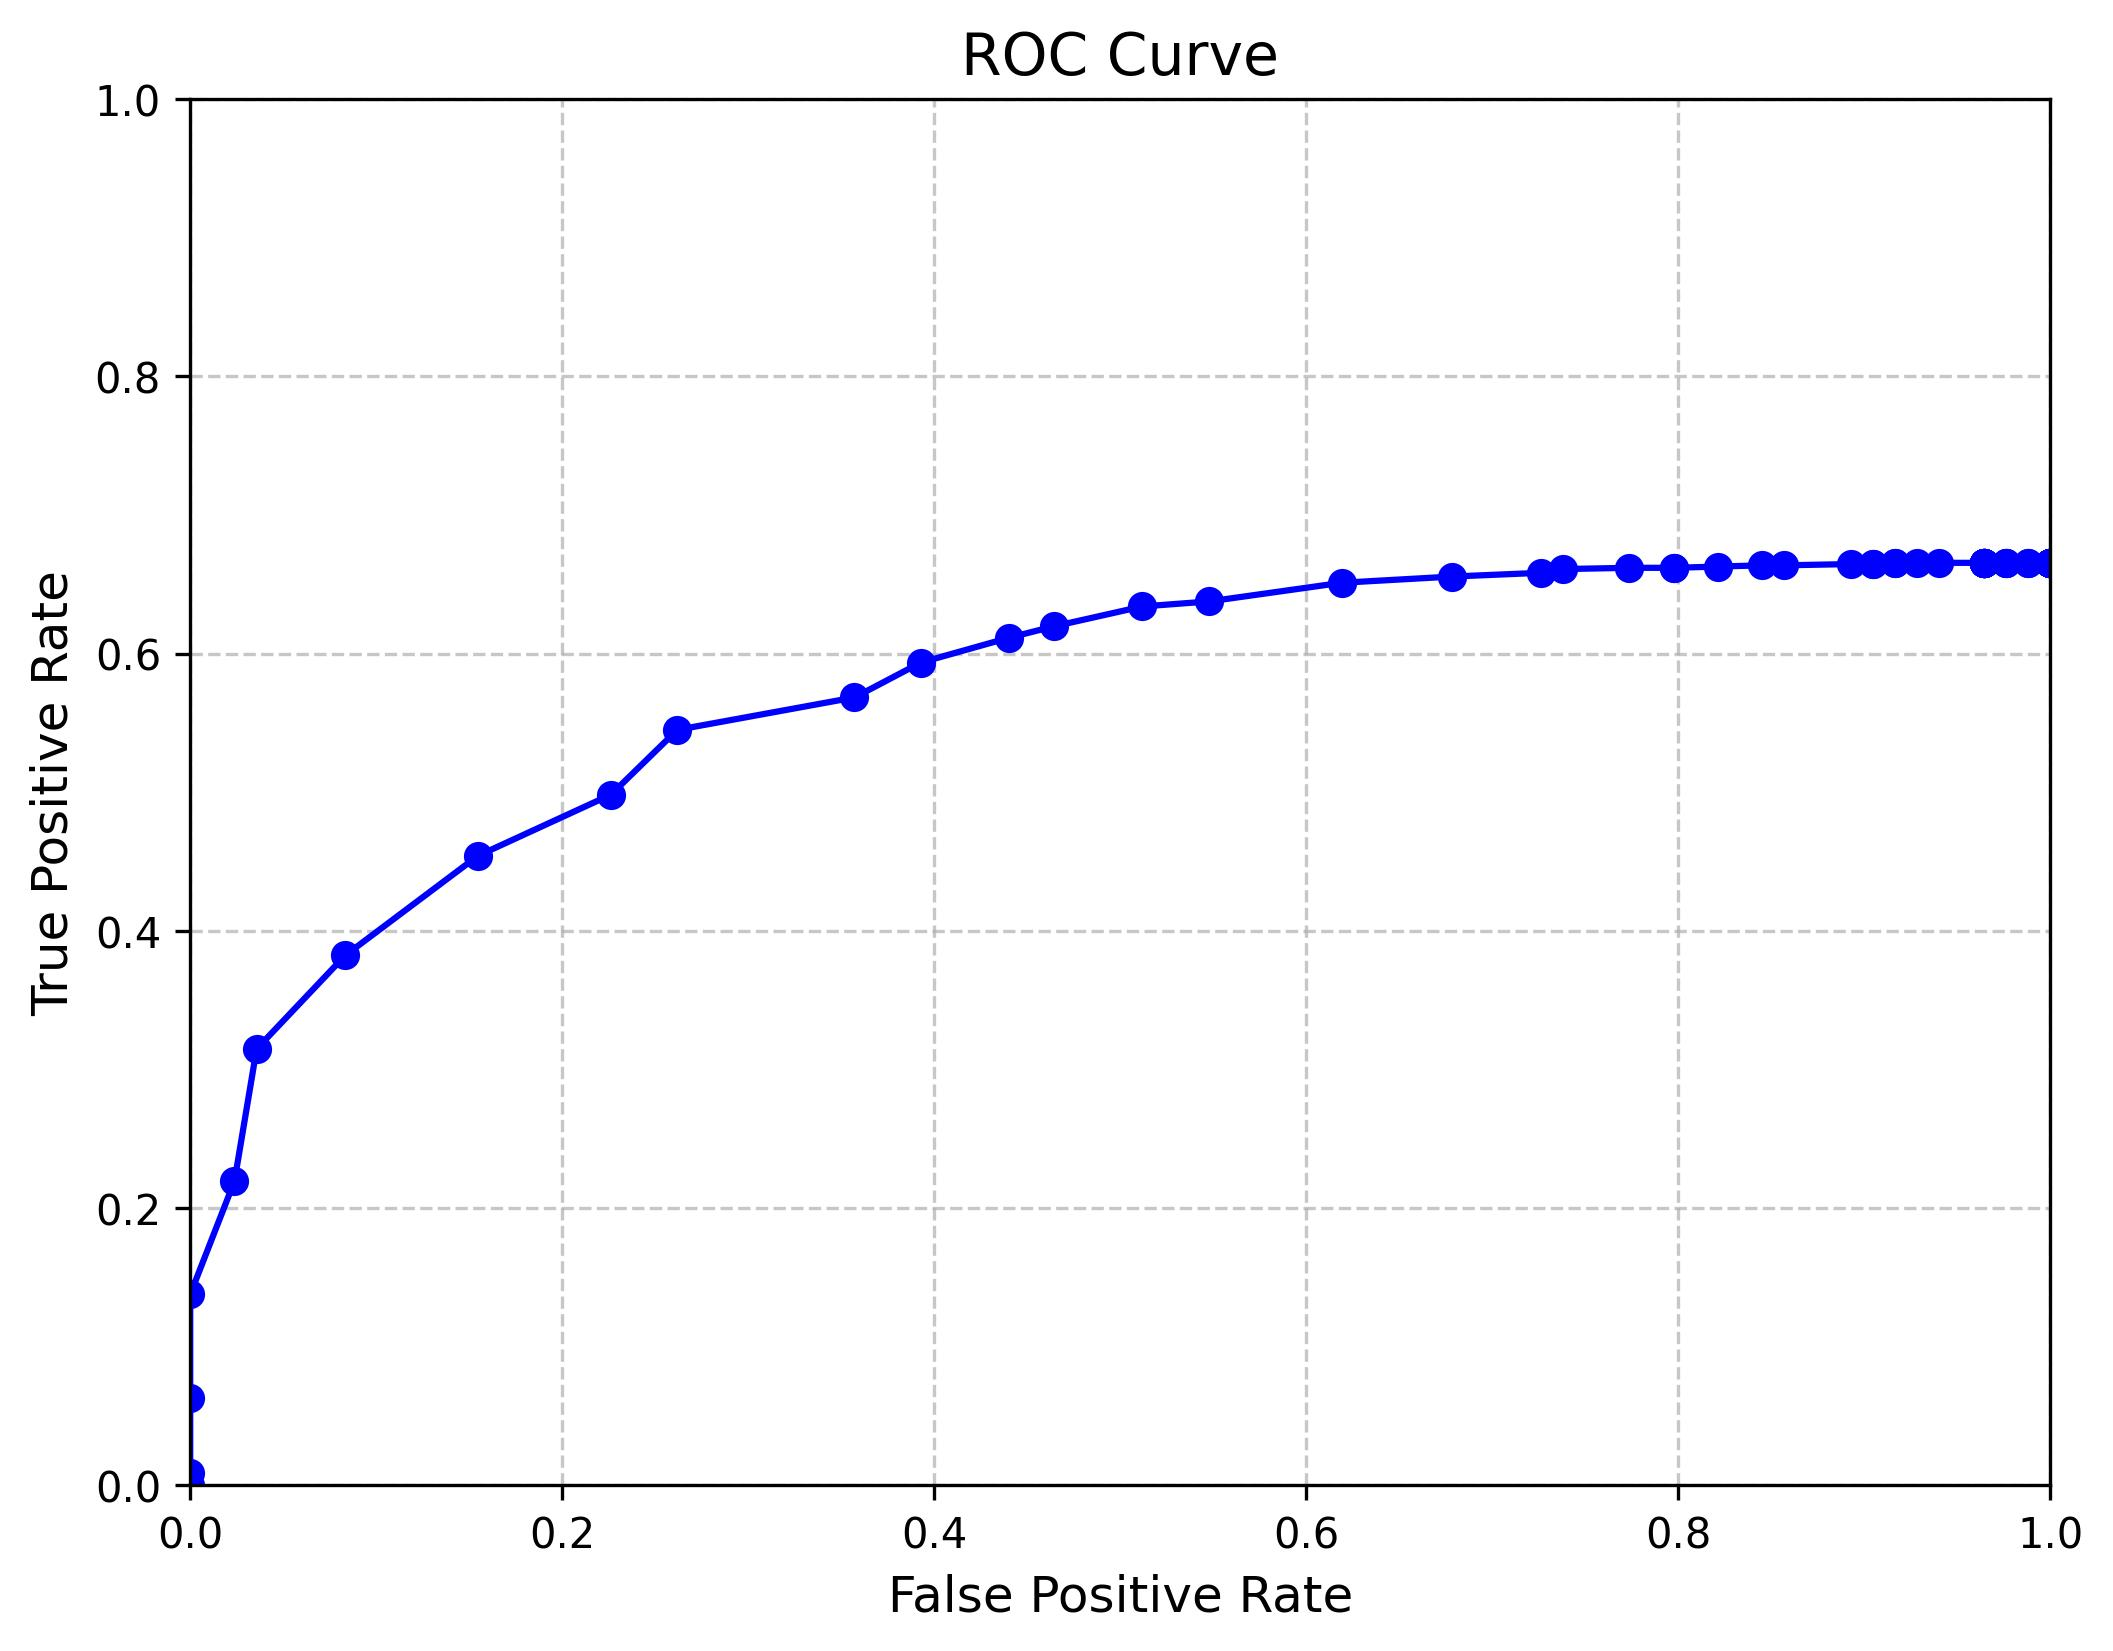
\includegraphics[width=0.8\textwidth]{../ROC_Curve.jpg}
    \caption{ROC curve for intruder detection (fa2\_H training, fb\_H testing, 95\% variance threshold).}
    \label{fig:roc}
\end{figure}
\end{document}
